\chapter{Introduction}

\section{Sujet et stratégie}

Le \textbf{Wave Function Collapse} (WFC) en modèle \textit{overlapping} \cite{gumin2016wfc} prend un échantillon $S$ et un paramètre $N$, et produit une grille $G$ telle que tout sous-bloc $N \times N$ de $G$ apparaisse dans $S$. L'algorithme combine deux primitives : \textit{sélection min-entropie} (choisir la cellule la plus contrainte) et \textit{propagation BFS} (intersecter les contraintes des voisins). Il est intrinsèquement séquentiel sur l'arbre de décisions, mais offre du parallélisme \emph{intra-niveau} : le scan d'entropie et la propagation BFS niveau-synchrone se chunkent sur threads.

\begin{figure}[H]
\centering
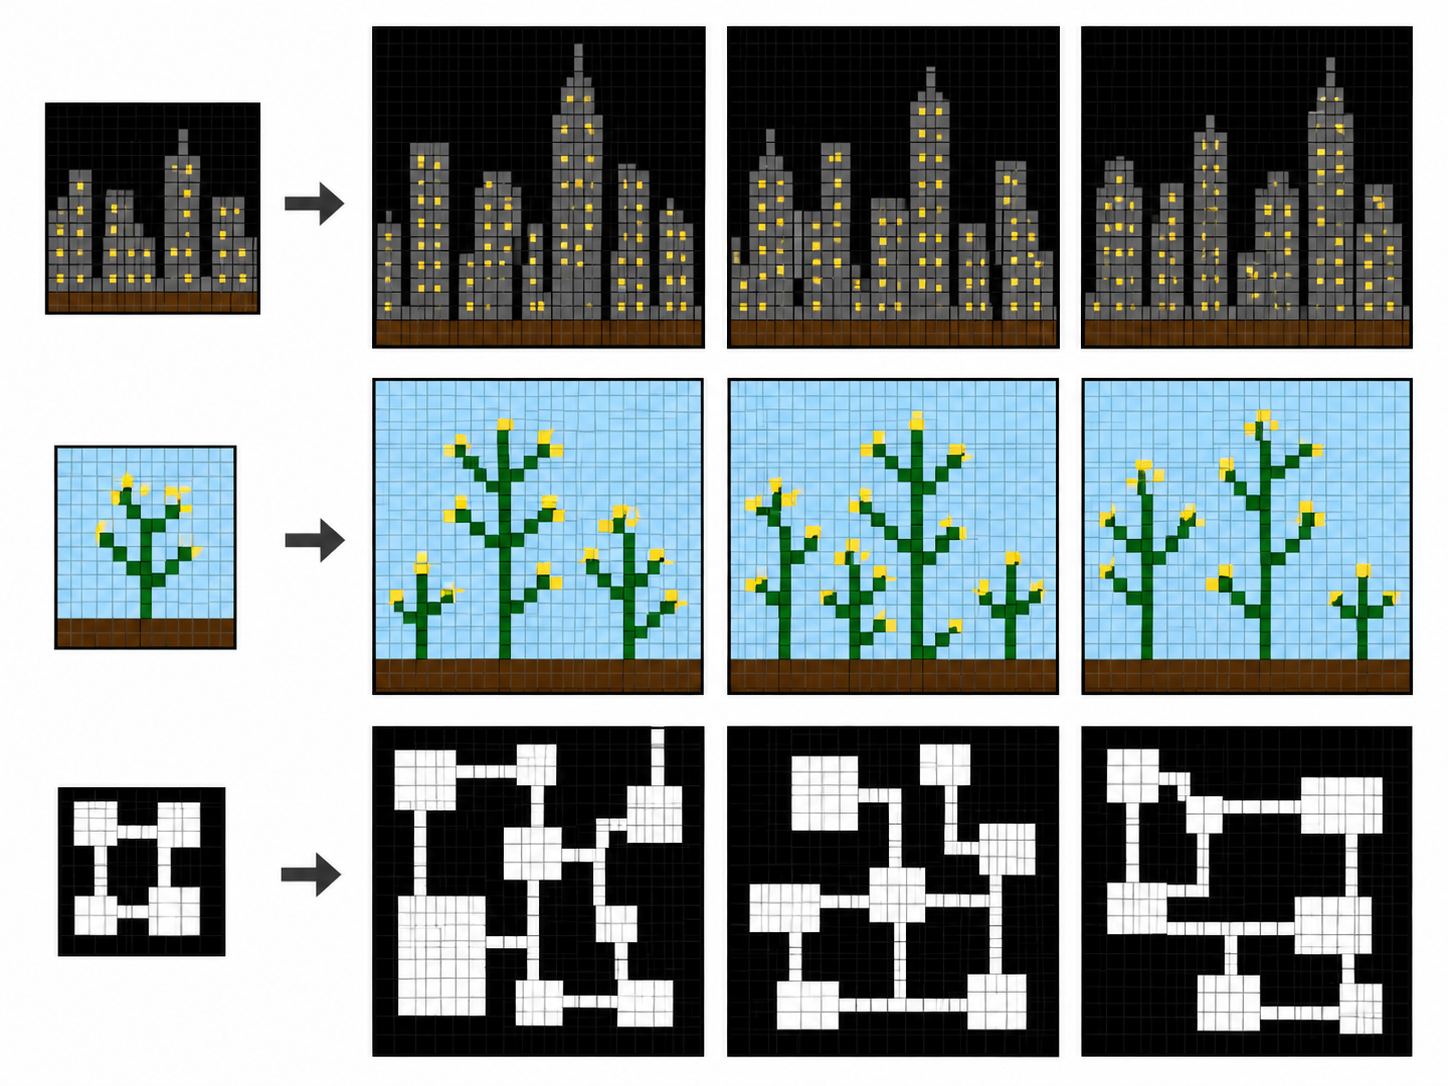
\includegraphics[width=0.85\linewidth]{results/figures/schemas/wfc_paper_outputs.png}
\caption{Sorties WFC à partir de petits échantillons : skyline urbain, plante, dungeon binaire. Chaque ligne montre l'input à gauche et trois sorties générées avec des seeds différents.}
\label{fig:wfc_paper_outputs}
\end{figure}

\subsection{Stratégie d'implémentation}

Trois cibles incrémentales :
\begin{enumerate}
    \item \textbf{Solveur série} (\texttt{wfc\_serial}) : référence algorithmique, bitsets packés sur \texttt{uint64\_t}, BFS niveau-synchrone, jitter d'entropie déterministe SplitMix64.
    \item \textbf{Backend OpenMP} (\texttt{wfc\_omp}) : API \texttt{\#pragma omp task} explicite. Sélection min-entropie chunkée + réduction ordonnée. Propagation pilotée par une seule région \texttt{parallel} (les barrières par niveau seraient catastrophiques sur 8000 niveaux BFS).
    \item \textbf{Backend Kokkos} (\texttt{wfc\_kokkos}) : même code source pour CPU OpenMP et GPU CUDA, branche compile-time \texttt{kHostOnly} pour le zero-copy CPU vs \texttt{deep\_copy} GPU.
\end{enumerate}

Tous trois produisent un output \textbf{bit-identique} pour un même seed, vérifié par hash SHA-256. Cette contrainte oriente plusieurs choix : RNG stateless, réduction en ordre de chunk fixe, atomics commutatives.

Quatre extensions opt-in : parallel-attempts, symétries D4, backtracking delta-encodé, démo Unreal Engine 5.7.

\subsection{Problèmes rencontrés}

Trois difficultés majeures pendant le développement, traitées dans les chapitres correspondants :

\begin{itemize}
    \item \textbf{Régression OMP fork/join} : ouvrir une région \texttt{parallel} par niveau BFS coûte $\sim 50$ µs $\times$ 8000 niveaux $= 400$ ms d'overhead pur, plus que le travail utile. Résolu par une seule région \texttt{parallel} ouverte avec \texttt{single} pilotant les niveaux (Section~\ref{sec:omp:propagate}).
    \item \textbf{Kokkos finalize crash} : Views cachées dans \texttt{thread\_local} désallouées \emph{après} le \texttt{finalize} de Kokkos. Résolu par \texttt{push\_finalize\_hook} (Section~\ref{sec:kokkos:cleanup}).
    \item \textbf{GPU plus lent que CPU} : sur GH200, transferts H$\leftrightarrow$D par appel à \texttt{propagate} dominent (16 GB pour 256$\times$256). Documenté comme limite structurelle, pas un bug (Section~\ref{sec:res:kokkos}).
\end{itemize}

\subsection{Analyse de performance}

220+ runs SLURM sur Romeo (EPYC 9654, 192 cœurs, 8 NUMA), avec variation systématique de :

\begin{itemize}
    \item \textbf{Taille de grille} : 32$\times$32 à 256$\times$256.
    \item \textbf{Sample (input)} : binary\_L11 (référence), terrain\_L33 (multi-valeurs riche), smooth\_N3 (cas pathologique).
    \item \textbf{Threads OpenMP} : 1, 2, 4, 8, 16, 32, 64, 192.
    \item \textbf{Backend} : serial, omp, kokkos (CPU + GPU).
\end{itemize}

Métriques calculées : speedup, efficacité parallèle, throughput, heatmap taille$\times$threads, fit Amdahl par configuration. Détails Chapitre~\ref{chap:resultats}.

\textbf{Speedup peak observé : 8.23$\times$ à 16 threads sur 256$\times$256 binary\_L11.}

\section{Organisation du rapport}

\begin{itemize}
    \item Chap.~\ref{chap:preliminaires} : préliminaires (complexité, OpenMP, Kokkos, métriques).
    \item Chap.~\ref{chap:probleme_wfc} : formalisation du problème WFC overlapping.
    \item Chap.~\ref{chap:approche} : algorithme séquentiel.
    \item Chap.~\ref{chap:implementation} : implémentation C++ (Bitset, Wave, CMake).
    \item Chap.~\ref{chap:openmp} : backend OpenMP, optims A/B.
    \item Chap.~\ref{chap:kokkos} : backend Kokkos GPU-portable.
    \item Chap.~\ref{chap:extensions} : extensions opt-in (parallel-attempts, D4, backtrack, UE5).
    \item Chap.~\ref{chap:protocole} : protocole expérimental.
    \item Chap.~\ref{chap:resultats} : résultats et analyse (speedup, scaling, Amdahl, varying input/config).
    \item Chap.~\ref{chap:limites} : limites et pistes (NUMA partitioning, batch GPU, PQ incrémentale).
    \item Chap.~\ref{chap:conclusion} : bilan.
\end{itemize}
